\newpage

\section{Предложенный метод и его корректность}
В данной работе LoRA применяется к задаче классификации. Структура обновления весов при использовании LoRA адаптера описана в таблице~\ref{table:1},
\begin{table}[ht!]
    \centering
\begin{tabular}{ | c | c| } 
 \hline
  Fine tuning & LoRA fine tuning\\ 
 \hline
 $W_{upd} = W + \Delta W$ & $W_{upd} = W + AB$\\ 
 $\hat{y} = xW_{upd}= x(W + \Delta W)$ & $\hat{y} = xW_{upd}= x(W + AB)$\\
 $\hat{y} = xW + x\Delta W$ & $\hat{y} = xW + xAB$ \\
 \hline
\end{tabular}
    \caption{Структура обновления весов при использовании LoRA адаптера}
    \label{table:1}
\end{table}

где~$W \in \mathbb{R}^{d \times k}$~--- предобученные веса,~$\Delta W \in \mathbb{R}^{d \times k}$~--- матрица обновленных весов.~$\Delta W$ приближается с помощью метода LoRA произведением~$AB$, где~$A \in \mathbb{R}^{d \times r}$,~$B \in \mathbb{R}^{r \times k}$ и~$r$~--- ранг матрицы, являющийся гиперпараметром модели. Здесь~$A \sim \mathcal{N}(0,\,\sigma^{2})$ и~$B = [0]_{r \times k}$. 

\subsection{Состоятельность предложенной модели}
Состоятельность модели трансформер была доказана в работе~\cite{lee2023mathematical}. Доказательство приведено для задачи классификации:
\begin{theorem}
\label{theorem:1}
Будем считать, что: 
\begin{enumerate}
    \item Задана модель с набором параметров~$\Theta^*$, генерирующая эмпирическое распределение данных~$P_{model}(\cdot, \Theta^*)$, которое аппроксимирует истинное распределение данных~$P_{true}$ с минимальным расхождением по KL-дивергенции: 
    \begin{equation}
    \label{eq:1}
    \exists \Theta^*: \Theta^* = \argmin _\Theta D_{KL}(P_{true} \mid\mid P_{model}(\cdot, \Theta)),
    \end{equation}
     \item При увеличении размера выборки~$\hat{V}$ эмпирическое распределение данных $P_{model}(\cdot, \Theta^*)$ приближается к истинному распределению, генерирующему данные.
     \item Функция ошибки~$\mathscr{L}(\Theta)$~--- непрерывная, дифференцируемая. Где
\end{enumerate}
\begin{equation}
\label{eq:2.1}
\mathscr{L}(\Theta) = -\frac{1}{\mid \hat{V} \mid}\sum_{X_i \in \hat{V}} \sum_{c_i \in [N_c]} \log \left(P_{\Phi_0+\Theta}\left(c_i \mid X_i\right)\right).
\end{equation}

Тогда минимизация функции потерь~$\mathscr{L}(\Theta)$ приводит к состоятельной оценке истинного распределения, порождающего данные. Т.е.: 
\begin{equation}
\label{eq:2.2}
    \lim_{\mid\hat{V}\mid\to\infty} \argmin _\Theta \mathscr{L}(\Theta) = \Theta^*.
\end{equation}

\end{theorem}
\renewcommand\qedsymbol{$\blacksquare$}
\begin{proof}
В силу равномерной сходимости функции потерь и силу утверждения~\ref{statement:1} из статьи~\cite{donini2018empirical}, которое приведено в приложении:
минимум~$\mathscr{L}(\Theta)$ стремится к минимуму ожидаемого риска~\begin{equation}
    R_{exp}=\E _{X_i \sim P_{true}} [\mathscr{L}(X_i; \Theta)],
\end{equation}при размере $\hat{V}$ стремящемся к бесконечности:
\begin{equation}
\label{eq:3.1}
\begin{aligned}
\lim_{\mid\hat{V}\mid\to\infty}  \argmin _\Theta \mathscr{L}(\Theta)  = \argmin _\Theta R_{exp} = \argmin _\Theta \E _{X_i \sim P_{true}} [\mathscr{L}(X_i; \Theta)].
\end{aligned}
\end{equation}
Достаточно доказать 
\begin{equation}
\label{eq:3.2}
\begin{aligned}
\argmin _\Theta \E _{X_i \sim P_{true}} [\mathscr{L}(X_i; \Theta)] = \Theta^*.
\end{aligned}
\end{equation}
Подставим значение функции потерь:
\begin{equation}
\label{eq:3.3}
\begin{aligned}
\argmin _\Theta \E _{X_i \sim P_{true}} [\mathscr{L}(X_i; \Theta)] =&\\
\argmin _\Theta \E _{X_i \sim P_{true}}[\sum_{c_i \in [N_c]} \log \left(P_{\Phi_0+\Theta}\left(c_i \mid X_i; \Theta)\right]\right).
\end{aligned}
\end{equation}

В силу определения KL-дивергенции,
\begin{equation}
\label{eq:4}
D_{KL}(P || Q)=\int_{-\infty}^{\infty} p(x) \log \left(\frac{p(x)}{q(x)}\right) dx = \E _{x \sim p(x)}[\log \left(\frac{p(x)}{q(x)}\right)],
\end{equation}
верно
\begin{equation}
\label{eq:3.4}
\begin{aligned}
\argmin _\Theta \E _{X_i\in P_{true}}[\sum_{c_i \in [N_c]} \log \left(P_{\Phi_0+\Delta \Phi(\Theta)}\left(c_i \mid X_i\right)\right] =&\\
    \argmin _\Theta D_{KL}(P_{true}\mid\mid P_{model}(\Theta)) =&~\Theta^*,
\end{aligned}
\end{equation}
Последнее равенство справедливо по условию. И оценка \begin{equation}
  \argmin _\Theta \E \mathscr{L}(\Theta)~\textrm{является состоятельной оценкой распределения}~P_{true}.  
\end{equation}
\end{proof}

\subsection{О применимости LoRA к задаче классификации}
Докажем, что LoRA применима к задаче классификации. Для решения задачи классификации с помощью BERT~\cite{vaswani2017attention} требуется не более чем дополнительный~$\operatorname{softmax}$ слой после BERT~\cite{sun2019fine}: 
\begin{equation}
\label{eq:5}
\begin{aligned}
p(c \mid \mathbf{x})&=\operatorname{softmax}(W^T \mathbf{x})\\
\hat{\mathbf{y}}&=\operatorname{softmax}\left(W^T \mathbf{x}\right)=\frac{\exp \left(W^T \mathbf{x}\right)}{\sum_{i=1}^k \exp \left(W^T \mathbf{x}\right)_i},
\end{aligned}
\end{equation}
где~$\mathbf{x}$~--- это выходной результат последнего слоя BERT, а $W$~--- матрица весов.
\begin{figure}[ht!]
    \centering
    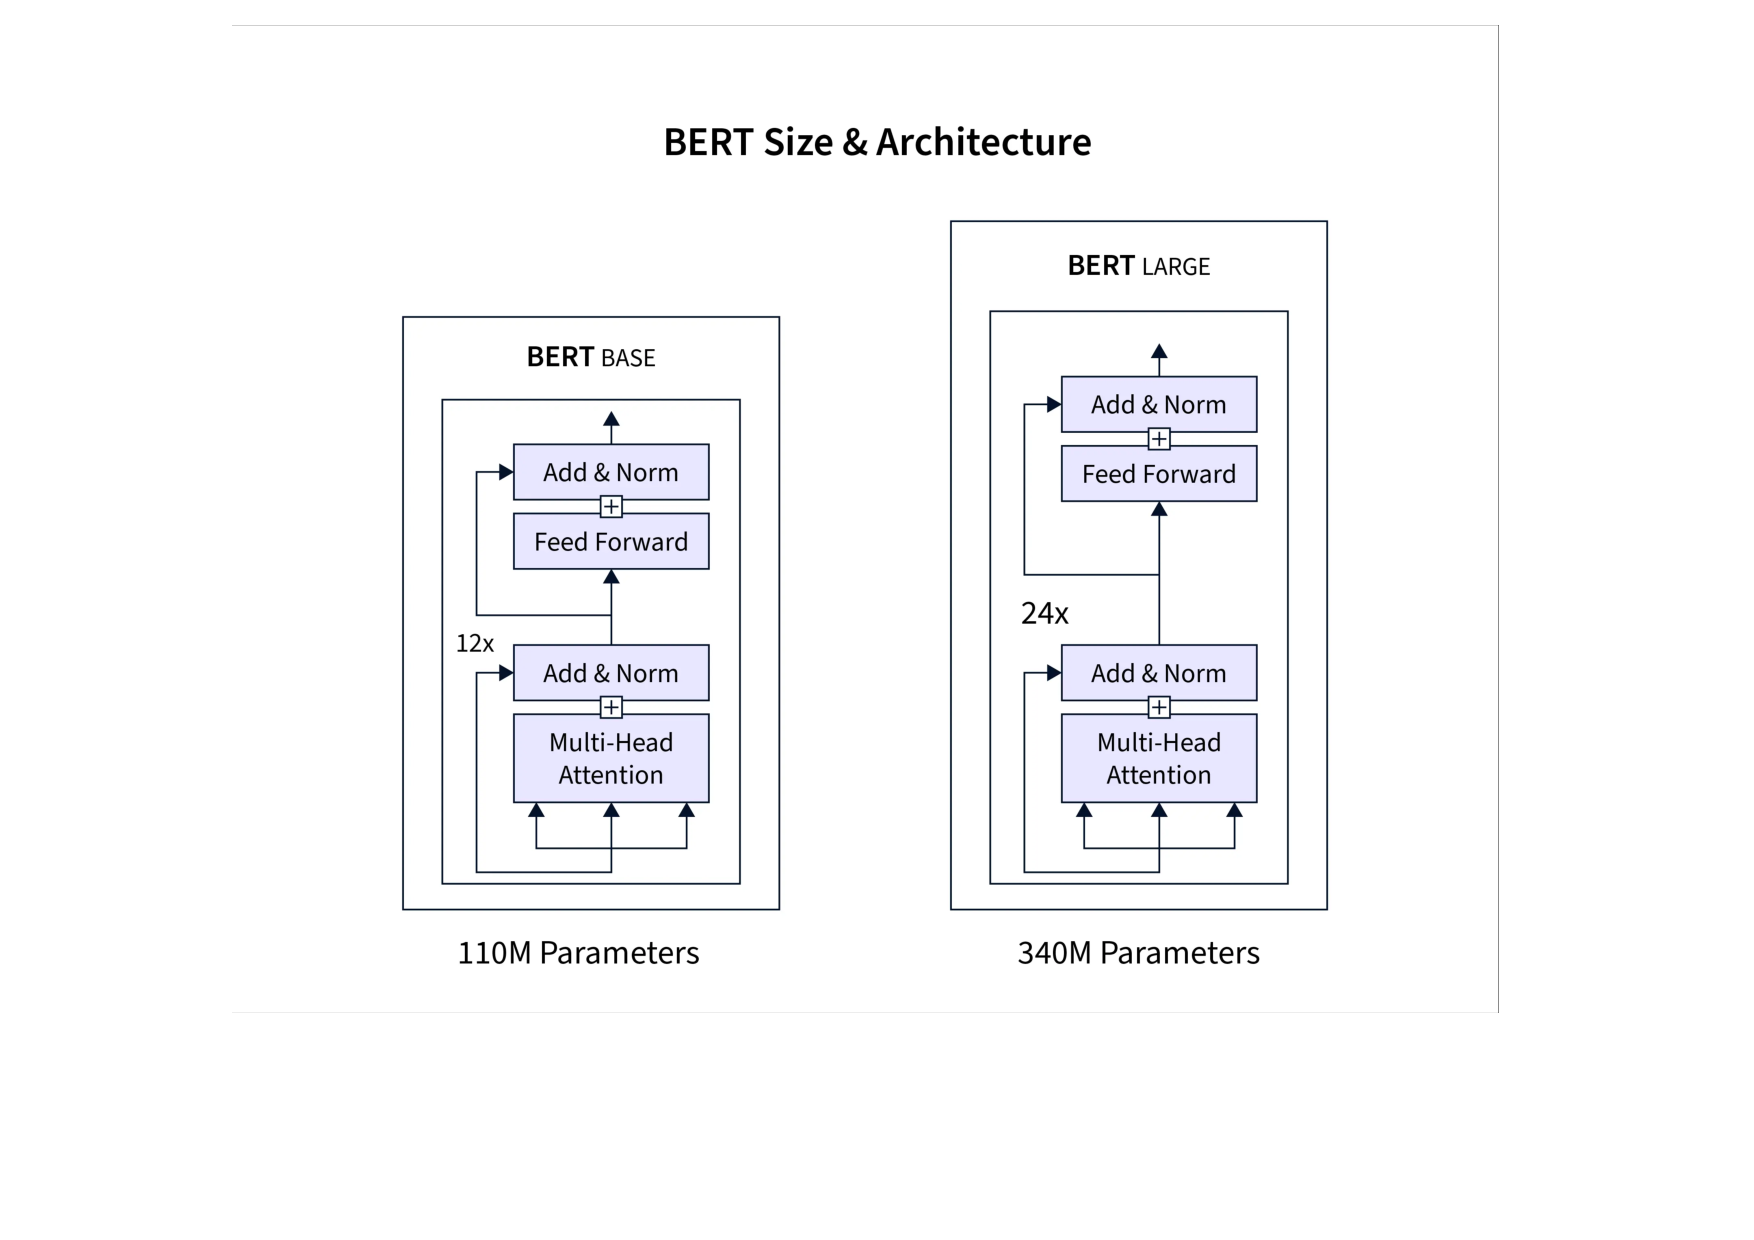
\includegraphics[width=1.0\textwidth]{images/bert_architecture copy.pdf}
    \caption{Архитектура модели BERT}
    \label{fig:1}
\end{figure}
Структура BERT представлена на рис.~\ref{fig:1}, где, согласно~\cite{thickstun2021transformer}, слой внимания~(англ. attention):
\begin{equation}
\begin{aligned}
Q^{(h)}\left(\mathbf{x}_i\right)&=W_{h, q}^T \mathbf{x}_i,\\
K^{(h)}\left(\mathbf{x}_i\right)&=W_{h, k}^T \mathbf{x}_i,  \quad W_{h, q}, W_{h, k}, W_{h, v} \in \mathbb{R}^{d \times k},\\
V^{(h)}\left(\mathbf{x}_i\right)&=W_{h, v}^T \mathbf{x}_i,
\end{aligned}
\end{equation}
\begin{equation}
\begin{aligned}
\alpha_{i,j}^{(h)}=&\operatorname{softmax}_j\left(\frac{\left\langle Q^{(h)}\left(\mathbf{x}_i\right), K^{(h)}\left(\mathbf{x}_j\right)\right\rangle}{\sqrt{k}}\right)V^{(h)}\left(\mathbf{x}_j\right), \\
\mathbf{u}_i^{\prime}=&\sum_{h=1}^H W_{c, h}^T \sum_{j=1}^n \alpha_{i, j}^{(h)}, \\
\end{aligned}
\end{equation}
где $Q^{(h)}\left(\mathbf{x}_i\right), K^{(h)}\left(\mathbf{x}_i\right), V^{(h)}\left(\mathbf{x}_i\right)$~--- линейные проекции входного вектора $\mathbf{x}$ запрос, ключ, значение~(англ. Query, Key, Value) и $\alpha_{i,j}^{(h)}$~--- вектор внимания, $\mathbf{u}_i^{\prime}$~--- выходная матрица слоя attention такого же размера, как и входная $\mathbf{x}_i$~\cite{vaswani2017attention}.

Нормализация по слою~(англ. Layer normalization)~--- нормализует активации предыдущего слоя для каждого входа в партиции~(англ. batch) независимо друг от друга, а не по всей партиции, как при batch нормализации. То есть, применяет преобразование, которое поддерживает среднее в пределах каждого входа близким к 0 и стандартное отклонение активации близким к 1~\cite{ba2016layer}.
\begin{equation}
\begin{aligned}
&\mathbf{u}_i=\operatorname{LayerNorm}\left(\mathbf{x}_i+\mathbf{u}_i^{\prime} ; \gamma_1, \beta_1\right), \\
\end{aligned}
\end{equation}
Нормализация по слою может быть переписана в соответствии с~\cite{ba2016layer} следующим образом:
\begin{equation}
\begin{aligned}
& \operatorname{LayerNorm}(\mathbf{z} ; \gamma, \beta)=\gamma \frac{\left(\mathbf{z}-\mu_{\mathbf{z}}\right)}{\sigma_{\mathbf{z}}}+\beta, \\
& \gamma, \beta \in \mathbb{R}^k . \\
& \mu_{\mathbf{z}}=\frac{1}{k} \sum_{i=1}^k \mathbf{z}_i, \quad \sigma_{\mathbf{z}}=\sqrt{\frac{1}{k} \sum_{i=1}^k\left(\mathbf{z}_i-\mu_{\mathbf{z}}\right)^2} . \\
&
\end{aligned}
\end{equation}
Сеть прямого распространения~(англ. Feed Forward Network) представляет собой двухслойную нейронную сеть с активацией ReLU:
\begin{equation}
\begin{aligned}
& \mathbf{z}_i^{\prime}=W_2^T \operatorname{ReLU}\left(W_1^T \mathbf{u}_i + b_1\right) + b_2. \\
\end{aligned}
\end{equation}
%пояснить!
Нормализация по слою:
\begin{equation}
\begin{aligned}
\mathbf{z}_i=\text { LayerNorm }\left(\mathbf{u}_i+\mathbf{z}_i^{\prime} ; \gamma_2, \beta_2\right) \text {, }
\end{aligned}
\end{equation}


\begin{theorem}
В рамках задачи классификации, при заданных условиях:
\begin{enumerate}
    \item Модель семейства BERT с указанной выше математической структурой и дополнительным слоем 
    \begin{equation}
    \label{eq:6}
        \hat{\mathbf{y}}=\operatorname{softmax}\left(W_{upd}^T \mathbf{x}\right)=\frac{\exp \left(W_{upd}^T \mathbf{x}\right)}{\sum_{i=1}^k \exp \left(W_{upd}^T \mathbf{x}\right)_i},
    \end{equation}
    где 
    \begin{equation}
    \label{eq:7}
    W_{upd} =\underset{(d \times k) }{W} + \underset{(d \times k)}{\Delta W},
    \end{equation}
    и~$x$~---это выходной результат BERT,~$W$~--- матрица весов,~$\Delta W$~--- матрица обновленных весов.
    \item  Данная модель BERT без дополнительного слоя также корректно работает с аппроксимацией 
    \begin{equation}
    \label{eq:8}
    \underset{(d \times k)}{\Delta W} = \underset{(d \times r)}{ A} \times \underset{(r \times k)}{B},
    \end{equation}
    \item Условия теоремы выполняются~\ref{theorem:1}.~(можно считать данную модель состоятельной).
\end{enumerate}
Тогда можно утверждать, что при~\eqref{eq:8} заданная модель BERT с дополнительным слоем гарантирует корректную выходную матрицу.
\end{theorem}
\renewcommand\qedsymbol{$\blacksquare$}
\begin{proof} 
Докажем, что выход из дополнительного слоя корректен. По дистрибутивному свойству сложения матриц и ассоциативному свойтсву произведения матриц: 
\begin{equation}
\label{eq:9}
\begin{aligned}
\hat{\mathbf{y}} = \operatorname{softmax}\left(W_{upd}^T \mathbf{x}\right) =
\operatorname{softmax}\left((W + \Delta W)^T \mathbf{x}\right) =\\ \\
= \frac{\exp \left(W^T \mathbf{x} + \Delta W^T \mathbf{x}\right)}{\sum_{i=1}^k \exp \left(W^T \mathbf{x} + \Delta W^T \mathbf{x}\right)_i}=\\ \\
= \frac{\exp \left(W^T \mathbf{x}\right) \exp \left(\Delta W^T \mathbf{x}\right)}{\sum_{i=1}^k \exp \left(W^T \mathbf{x}\right)_i \exp \left(\Delta W^T \mathbf{x}\right)_i},
\end{aligned}
\end{equation} 
где~$\mathbf{x}$~--- выходная матрица последнего слоя BERT.~$\mathbf{x}$ корректна по условию. В предложенной модели с использованием LoRA:
\begin{equation}
\label{eq:10}
\begin{aligned}
\hat{\mathbf{y}} = \operatorname{softmax}\left(W_{upd} \mathbf{x}\right) =
\operatorname{softmax}\left((W + AB)^T \mathbf{x}\right) =\\ \\
= \frac{\exp \left(W^T \mathbf{x} + (AB)^T \mathbf{x}\right)}{\sum_{i=1}^k \exp \left(W^T \mathbf{x} + (AB)^T \mathbf{x}\right)_i}=\\ \\
= \frac{\exp \left(W^T \mathbf{x}\right) \exp \left((AB)^T \mathbf{x}\right)}{\sum_{i=1}^k \exp \left(W^T \mathbf{x}\right)_i \exp \left((AB)^T \mathbf{x}\right)_i},
\end{aligned}
\end{equation} 
где~$\mathbf{x}$ также выходная матрица BERT с LoRA и~$\mathbf{x}$ корректна по условию. 

Так как финальные размерности остались неизменными, как и~$W^T\mathbf{x}$, легко заметить: 
\begin{equation}
\label{eq:11}
\begin{aligned}
 \underset{(k \times d)}{\Delta W^T} \times \mathbf{x} = u\\
(\underset{(d \times r)}{A} \times \underset{(r \times k)}{B})^T \times \mathbf{x} = (\underset{(k \times r)}{B^T} \times \underset{(r \times d)}{A^T}) \times \mathbf{x} = u^*.
\end{aligned}
\end{equation}
Так как~\eqref{eq:10}, можно заключить что~${u^*} = {u}$ и является корретной матрицей, а следовательно предложенная модель работает корректно.
\end{proof}
